\documentclass[10pt]{article}
\usepackage{amsmath,amssymb}
\usepackage{graphicx}
\usepackage{longtable}
\usepackage{array}
\usepackage[hidelinks]{hyperref}
\usepackage[margin=0.9in]{geometry}
\usepackage[numbers]{natbib}
\graphicspath{{../paper/}}
% Generated by reapschema.report; do not edit.
% config: paper
% results-hash: 417e9e5c49a26c543e409a6946ec791e31a37543321074b43a488199275cfc8d
\newcommand{\AccCurrentCleanEeiMare}{31.2}
\newcommand{\AccCurrentCleanEeiMedian}{22.8}
\newcommand{\AccCurrentCleanEeiQHigh}{100.1}
\newcommand{\AccCurrentCleanEeiQLow}{2.0}
\newcommand{\AccCurrentCleanEeiShareTen}{74.9}
\newcommand{\AccCurrentCleanResMare}{0.4}
\newcommand{\AccCurrentCleanResMedian}{0.33}
\newcommand{\AccCurrentCleanResQHigh}{0.98}
\newcommand{\AccCurrentCleanResQLow}{0.03}
\newcommand{\AccCurrentCleanResShareTen}{0.0}
\newcommand{\AccCurrentUnvalidatedEeiMare}{36.5}
\newcommand{\AccCurrentUnvalidatedEeiMedian}{25.5}
\newcommand{\AccCurrentUnvalidatedEeiQHigh}{228.4}
\newcommand{\AccCurrentUnvalidatedEeiQLow}{2.1}
\newcommand{\AccCurrentUnvalidatedEeiShareTen}{76.6}
\newcommand{\AccCurrentUnvalidatedResMare}{8.3}
\newcommand{\AccCurrentUnvalidatedResMedian}{0.40}
\newcommand{\AccCurrentUnvalidatedResQHigh}{69.43}
\newcommand{\AccCurrentUnvalidatedResQLow}{0.04}
\newcommand{\AccCurrentUnvalidatedResShareTen}{13.7}
\newcommand{\AccCurrentValidatedEeiMare}{33.4}
\newcommand{\AccCurrentValidatedEeiMedian}{23.8}
\newcommand{\AccCurrentValidatedEeiQHigh}{130.3}
\newcommand{\AccCurrentValidatedEeiQLow}{2.0}
\newcommand{\AccCurrentValidatedEeiShareTen}{75.5}
\newcommand{\AccCurrentValidatedResMare}{1.0}
\newcommand{\AccCurrentValidatedResMedian}{0.35}
\newcommand{\AccCurrentValidatedResQHigh}{1.24}
\newcommand{\AccCurrentValidatedResQLow}{0.03}
\newcommand{\AccCurrentValidatedResShareTen}{2.6}
\newcommand{\AccDatesCleanEeiMare}{30.7}
\newcommand{\AccDatesCleanEeiMedian}{22.5}
\newcommand{\AccDatesCleanEeiQHigh}{97.3}
\newcommand{\AccDatesCleanEeiQLow}{2.0}
\newcommand{\AccDatesCleanEeiShareTen}{75.0}
\newcommand{\AccDatesCleanResMare}{0.4}
\newcommand{\AccDatesCleanResMedian}{0.33}
\newcommand{\AccDatesCleanResQHigh}{0.98}
\newcommand{\AccDatesCleanResQLow}{0.03}
\newcommand{\AccDatesCleanResShareTen}{0.0}
\newcommand{\AccDatesNormCleanEeiMare}{23.1}
\newcommand{\AccDatesNormCleanEeiMedian}{15.2}
\newcommand{\AccDatesNormCleanEeiQHigh}{76.8}
\newcommand{\AccDatesNormCleanEeiQLow}{1.1}
\newcommand{\AccDatesNormCleanEeiShareTen}{63.9}
\newcommand{\AccDatesNormCleanResMare}{0.4}
\newcommand{\AccDatesNormCleanResMedian}{0.33}
\newcommand{\AccDatesNormCleanResQHigh}{0.98}
\newcommand{\AccDatesNormCleanResQLow}{0.03}
\newcommand{\AccDatesNormCleanResShareTen}{0.0}
\newcommand{\AccDatesNormReadCleanEeiMare}{21.5}
\newcommand{\AccDatesNormReadCleanEeiMedian}{14.5}
\newcommand{\AccDatesNormReadCleanEeiQHigh}{69.3}
\newcommand{\AccDatesNormReadCleanEeiQLow}{1.1}
\newcommand{\AccDatesNormReadCleanEeiShareTen}{61.9}
\newcommand{\AccDatesNormReadCleanResMare}{0.4}
\newcommand{\AccDatesNormReadCleanResMedian}{0.33}
\newcommand{\AccDatesNormReadCleanResQHigh}{0.98}
\newcommand{\AccDatesNormReadCleanResQLow}{0.03}
\newcommand{\AccDatesNormReadCleanResShareTen}{0.0}
\newcommand{\AccDatesNormReadUnvalidatedEeiMare}{27.9}
\newcommand{\AccDatesNormReadUnvalidatedEeiMedian}{16.3}
\newcommand{\AccDatesNormReadUnvalidatedEeiQHigh}{226.9}
\newcommand{\AccDatesNormReadUnvalidatedEeiQLow}{1.1}
\newcommand{\AccDatesNormReadUnvalidatedEeiShareTen}{64.7}
\newcommand{\AccDatesNormReadUnvalidatedResMare}{8.3}
\newcommand{\AccDatesNormReadUnvalidatedResMedian}{0.40}
\newcommand{\AccDatesNormReadUnvalidatedResQHigh}{69.43}
\newcommand{\AccDatesNormReadUnvalidatedResQLow}{0.04}
\newcommand{\AccDatesNormReadUnvalidatedResShareTen}{13.7}
\newcommand{\AccDatesNormReadValidatedEeiMare}{24.3}
\newcommand{\AccDatesNormReadValidatedEeiMedian}{15.2}
\newcommand{\AccDatesNormReadValidatedEeiQHigh}{102.0}
\newcommand{\AccDatesNormReadValidatedEeiQLow}{1.1}
\newcommand{\AccDatesNormReadValidatedEeiShareTen}{63.1}
\newcommand{\AccDatesNormReadValidatedResMare}{1.0}
\newcommand{\AccDatesNormReadValidatedResMedian}{0.35}
\newcommand{\AccDatesNormReadValidatedResQHigh}{1.24}
\newcommand{\AccDatesNormReadValidatedResQLow}{0.03}
\newcommand{\AccDatesNormReadValidatedResShareTen}{2.6}
\newcommand{\AccDatesNormUnvalidatedEeiMare}{29.5}
\newcommand{\AccDatesNormUnvalidatedEeiMedian}{17.2}
\newcommand{\AccDatesNormUnvalidatedEeiQHigh}{245.6}
\newcommand{\AccDatesNormUnvalidatedEeiQLow}{1.3}
\newcommand{\AccDatesNormUnvalidatedEeiShareTen}{66.7}
\newcommand{\AccDatesNormUnvalidatedResMare}{8.3}
\newcommand{\AccDatesNormUnvalidatedResMedian}{0.40}
\newcommand{\AccDatesNormUnvalidatedResQHigh}{69.43}
\newcommand{\AccDatesNormUnvalidatedResQLow}{0.04}
\newcommand{\AccDatesNormUnvalidatedResShareTen}{13.7}
\newcommand{\AccDatesNormValidatedEeiMare}{25.9}
\newcommand{\AccDatesNormValidatedEeiMedian}{16.2}
\newcommand{\AccDatesNormValidatedEeiQHigh}{117.2}
\newcommand{\AccDatesNormValidatedEeiQLow}{1.2}
\newcommand{\AccDatesNormValidatedEeiShareTen}{65.0}
\newcommand{\AccDatesNormValidatedResMare}{1.0}
\newcommand{\AccDatesNormValidatedResMedian}{0.35}
\newcommand{\AccDatesNormValidatedResQHigh}{1.24}
\newcommand{\AccDatesNormValidatedResQLow}{0.03}
\newcommand{\AccDatesNormValidatedResShareTen}{2.6}
\newcommand{\AccDatesUnvalidatedEeiMare}{36.1}
\newcommand{\AccDatesUnvalidatedEeiMedian}{25.0}
\newcommand{\AccDatesUnvalidatedEeiQHigh}{227.0}
\newcommand{\AccDatesUnvalidatedEeiQLow}{2.1}
\newcommand{\AccDatesUnvalidatedEeiShareTen}{76.6}
\newcommand{\AccDatesUnvalidatedResMare}{8.3}
\newcommand{\AccDatesUnvalidatedResMedian}{0.40}
\newcommand{\AccDatesUnvalidatedResQHigh}{69.43}
\newcommand{\AccDatesUnvalidatedResQLow}{0.04}
\newcommand{\AccDatesUnvalidatedResShareTen}{13.7}
\newcommand{\AccDatesValidatedEeiMare}{33.1}
\newcommand{\AccDatesValidatedEeiMedian}{23.5}
\newcommand{\AccDatesValidatedEeiQHigh}{130.3}
\newcommand{\AccDatesValidatedEeiQLow}{2.0}
\newcommand{\AccDatesValidatedEeiShareTen}{75.7}
\newcommand{\AccDatesValidatedResMare}{1.0}
\newcommand{\AccDatesValidatedResMedian}{0.35}
\newcommand{\AccDatesValidatedResQHigh}{1.24}
\newcommand{\AccDatesValidatedResQLow}{0.03}
\newcommand{\AccDatesValidatedResShareTen}{2.6}
\newcommand{\AccIntervalCleanEeiMare}{18.6}
\newcommand{\AccIntervalCleanEeiMedian}{12.1}
\newcommand{\AccIntervalCleanEeiQHigh}{60.3}
\newcommand{\AccIntervalCleanEeiQLow}{0.9}
\newcommand{\AccIntervalCleanEeiShareTen}{55.6}
\newcommand{\AccIntervalCleanResMare}{0.4}
\newcommand{\AccIntervalCleanResMedian}{0.33}
\newcommand{\AccIntervalCleanResQHigh}{0.98}
\newcommand{\AccIntervalCleanResQLow}{0.03}
\newcommand{\AccIntervalCleanResShareTen}{0.0}
\newcommand{\AccIntervalUnvalidatedEeiMare}{18.6}
\newcommand{\AccIntervalUnvalidatedEeiMedian}{12.1}
\newcommand{\AccIntervalUnvalidatedEeiQHigh}{60.3}
\newcommand{\AccIntervalUnvalidatedEeiQLow}{0.9}
\newcommand{\AccIntervalUnvalidatedEeiShareTen}{55.6}
\newcommand{\AccIntervalUnvalidatedResMare}{0.4}
\newcommand{\AccIntervalUnvalidatedResMedian}{0.33}
\newcommand{\AccIntervalUnvalidatedResQHigh}{0.98}
\newcommand{\AccIntervalUnvalidatedResQLow}{0.03}
\newcommand{\AccIntervalUnvalidatedResShareTen}{0.0}
\newcommand{\AccIntervalValidatedEeiMare}{18.6}
\newcommand{\AccIntervalValidatedEeiMedian}{12.1}
\newcommand{\AccIntervalValidatedEeiQHigh}{60.3}
\newcommand{\AccIntervalValidatedEeiQLow}{0.9}
\newcommand{\AccIntervalValidatedEeiShareTen}{55.6}
\newcommand{\AccIntervalValidatedResMare}{0.4}
\newcommand{\AccIntervalValidatedResMedian}{0.33}
\newcommand{\AccIntervalValidatedResQHigh}{0.98}
\newcommand{\AccIntervalValidatedResQLow}{0.03}
\newcommand{\AccIntervalValidatedResShareTen}{0.0}
\newcommand{\AccMetadataCleanEeiMare}{21.5}
\newcommand{\AccMetadataCleanEeiMedian}{14.5}
\newcommand{\AccMetadataCleanEeiQHigh}{69.3}
\newcommand{\AccMetadataCleanEeiQLow}{1.1}
\newcommand{\AccMetadataCleanEeiShareTen}{61.9}
\newcommand{\AccMetadataCleanResMare}{0.4}
\newcommand{\AccMetadataCleanResMedian}{0.33}
\newcommand{\AccMetadataCleanResQHigh}{0.98}
\newcommand{\AccMetadataCleanResQLow}{0.03}
\newcommand{\AccMetadataCleanResShareTen}{0.0}
\newcommand{\AccMetadataUnvalidatedEeiMare}{27.9}
\newcommand{\AccMetadataUnvalidatedEeiMedian}{16.3}
\newcommand{\AccMetadataUnvalidatedEeiQHigh}{226.9}
\newcommand{\AccMetadataUnvalidatedEeiQLow}{1.1}
\newcommand{\AccMetadataUnvalidatedEeiShareTen}{64.7}
\newcommand{\AccMetadataUnvalidatedResMare}{4.2}
\newcommand{\AccMetadataUnvalidatedResMedian}{0.35}
\newcommand{\AccMetadataUnvalidatedResQHigh}{1.36}
\newcommand{\AccMetadataUnvalidatedResQLow}{0.03}
\newcommand{\AccMetadataUnvalidatedResShareTen}{3.9}
\newcommand{\AccMetadataValidatedEeiMare}{21.5}
\newcommand{\AccMetadataValidatedEeiMedian}{14.5}
\newcommand{\AccMetadataValidatedEeiQHigh}{69.3}
\newcommand{\AccMetadataValidatedEeiQLow}{1.1}
\newcommand{\AccMetadataValidatedEeiShareTen}{61.8}
\newcommand{\AccMetadataValidatedResMare}{0.4}
\newcommand{\AccMetadataValidatedResMedian}{0.34}
\newcommand{\AccMetadataValidatedResQHigh}{0.99}
\newcommand{\AccMetadataValidatedResQLow}{0.03}
\newcommand{\AccMetadataValidatedResShareTen}{0.0}
\newcommand{\AccNettingCleanEeiMare}{31.2}
\newcommand{\AccNettingCleanEeiMedian}{22.8}
\newcommand{\AccNettingCleanEeiQHigh}{100.1}
\newcommand{\AccNettingCleanEeiQLow}{2.0}
\newcommand{\AccNettingCleanEeiShareTen}{74.9}
\newcommand{\AccNettingCleanResMare}{0.4}
\newcommand{\AccNettingCleanResMedian}{0.33}
\newcommand{\AccNettingCleanResQHigh}{0.98}
\newcommand{\AccNettingCleanResQLow}{0.03}
\newcommand{\AccNettingCleanResShareTen}{0.0}
\newcommand{\AccNettingUnvalidatedEeiMare}{36.5}
\newcommand{\AccNettingUnvalidatedEeiMedian}{25.5}
\newcommand{\AccNettingUnvalidatedEeiQHigh}{228.4}
\newcommand{\AccNettingUnvalidatedEeiQLow}{2.1}
\newcommand{\AccNettingUnvalidatedEeiShareTen}{76.6}
\newcommand{\AccNettingUnvalidatedResMare}{8.3}
\newcommand{\AccNettingUnvalidatedResMedian}{0.40}
\newcommand{\AccNettingUnvalidatedResQHigh}{69.43}
\newcommand{\AccNettingUnvalidatedResQLow}{0.04}
\newcommand{\AccNettingUnvalidatedResShareTen}{13.7}
\newcommand{\AccNettingValidatedEeiMare}{33.4}
\newcommand{\AccNettingValidatedEeiMedian}{23.8}
\newcommand{\AccNettingValidatedEeiQHigh}{130.3}
\newcommand{\AccNettingValidatedEeiQLow}{2.0}
\newcommand{\AccNettingValidatedEeiShareTen}{75.5}
\newcommand{\AccNettingValidatedResMare}{1.0}
\newcommand{\AccNettingValidatedResMedian}{0.35}
\newcommand{\AccNettingValidatedResQHigh}{1.23}
\newcommand{\AccNettingValidatedResQLow}{0.03}
\newcommand{\AccNettingValidatedResShareTen}{2.5}
\newcommand{\AccProductionMeterCleanEeiMare}{31.2}
\newcommand{\AccProductionMeterCleanEeiMedian}{22.8}
\newcommand{\AccProductionMeterCleanEeiQHigh}{100.1}
\newcommand{\AccProductionMeterCleanEeiQLow}{2.0}
\newcommand{\AccProductionMeterCleanEeiShareTen}{74.9}
\newcommand{\AccProductionMeterCleanResMare}{0.4}
\newcommand{\AccProductionMeterCleanResMedian}{0.33}
\newcommand{\AccProductionMeterCleanResQHigh}{0.98}
\newcommand{\AccProductionMeterCleanResQLow}{0.03}
\newcommand{\AccProductionMeterCleanResShareTen}{0.0}
\newcommand{\AccProductionMeterUnvalidatedEeiMare}{36.5}
\newcommand{\AccProductionMeterUnvalidatedEeiMedian}{25.5}
\newcommand{\AccProductionMeterUnvalidatedEeiQHigh}{228.4}
\newcommand{\AccProductionMeterUnvalidatedEeiQLow}{2.1}
\newcommand{\AccProductionMeterUnvalidatedEeiShareTen}{76.6}
\newcommand{\AccProductionMeterUnvalidatedResMare}{4.2}
\newcommand{\AccProductionMeterUnvalidatedResMedian}{0.35}
\newcommand{\AccProductionMeterUnvalidatedResQHigh}{1.36}
\newcommand{\AccProductionMeterUnvalidatedResQLow}{0.03}
\newcommand{\AccProductionMeterUnvalidatedResShareTen}{3.9}
\newcommand{\AccProductionMeterValidatedEeiMare}{33.4}
\newcommand{\AccProductionMeterValidatedEeiMedian}{23.8}
\newcommand{\AccProductionMeterValidatedEeiQHigh}{130.3}
\newcommand{\AccProductionMeterValidatedEeiQLow}{2.0}
\newcommand{\AccProductionMeterValidatedEeiShareTen}{75.5}
\newcommand{\AccProductionMeterValidatedResMare}{0.4}
\newcommand{\AccProductionMeterValidatedResMedian}{0.34}
\newcommand{\AccProductionMeterValidatedResQHigh}{0.99}
\newcommand{\AccProductionMeterValidatedResQLow}{0.03}
\newcommand{\AccProductionMeterValidatedResShareTen}{0.0}
\newcommand{\AnchorMinutes}{161}
\newcommand{\AnchorResponses}{2}
\newcommand{\AucBillDiffGrossNet}{0.80}
\newcommand{\AucBillDiffUnlabGrossNet}{0.65}
\newcommand{\AucOutlierTransposed}{0.54}
\newcommand{\AucPlausGeomNameplate}{0.97}
\newcommand{\AucPlausGrossNet}{0.96}
\newcommand{\AucPlausNameplate}{0.96}
\newcommand{\AucShapeTransposed}{0.57}
\newcommand{\AuditChainedHours}{150{,}153}
\newcommand{\AuditChainedShortfall}{730}
\newcommand{\AuditHoursDiscrepancy}{705}
\newcommand{\AuditHoursDiscrepancyPct}{0.47}
\newcommand{\AuditHoursPerRespondent}{50.7}
\newcommand{\AuditHoursPerResponse}{1.34}
\newcommand{\AuditImpliedHoursPerResponse}{1.3463}
\newcommand{\AuditImpliedResponsesPerRespondent}{37.6463}
\newcommand{\AuditProductHours}{150{,}178}
\newcommand{\AuditProductResponses}{112{,}054}
\newcommand{\AuditRespondents}{2{,}977}
\newcommand{\AuditResponses}{112{,}073}
\newcommand{\AuditResponsesDiscrepancy}{19}
\newcommand{\AuditResponsesPerRespondent}{37.64}
\newcommand{\AuditRoundedHoursPerResponse}{1.35}
\newcommand{\AuditRoundedResponsesPerRespondent}{37.65}
\newcommand{\AuditTotalHours}{150{,}883}
\newcommand{\AwardFitADCritical}{0.75}
\newcommand{\AwardFitADEei}{5.0}
\newcommand{\AwardFitADRes}{35.0}
\newcommand{\AwardFitNEei}{573}
\newcommand{\AwardFitNRes}{1{,}745}
\newcommand{\AwardShareAtSmallCap}{17}
\newcommand{\BandHighEdge}{20}
\newcommand{\BandHighIntervalPathMedian}{13}
\newcommand{\BandHighN}{860}
\newcommand{\BandHighNormMedian}{15}
\newcommand{\BandHighUndatedMedian}{17}
\newcommand{\BandLowEdge}{10}
\newcommand{\BandLowIntervalPathMedian}{15}
\newcommand{\BandLowN}{1{,}760}
\newcommand{\BandLowNormMedian}{19}
\newcommand{\BandLowUndatedMedian}{33}
\newcommand{\BandMidIntervalPathMedian}{9}
\newcommand{\BandMidN}{1{,}837}
\newcommand{\BandMidNormMedian}{13}
\newcommand{\BandMidUndatedMedian}{19}
\newcommand{\BaseBurden}{166}
\newcommand{\BaseFlagRate}{12}
\newcommand{\BaseMare}{8.2}
\newcommand{\BaseMareSe}{0.14}
\newcommand{\BaseSel}{9.2}
\newcommand{\BasisComstockIntervalMedian}{8}
\newcommand{\BasisComstockN}{2{,}239}
\newcommand{\BasisComstockNormMedian}{10}
\newcommand{\BasisComstockUndatedMedian}{19}
\newcommand{\BasisHypotheticalIntervalMedian}{18}
\newcommand{\BasisHypotheticalN}{2{,}218}
\newcommand{\BasisHypotheticalNormMedian}{20}
\newcommand{\BasisHypotheticalUndatedMedian}{27}
\newcommand{\CfgAreCap}{1}
\newcommand{\CfgBootstrap}{1{,}000}
\newcommand{\CfgBootstrapBlock}{3}
\newcommand{\CfgConfidence}{90}
\newcommand{\CfgCvrmseMax}{25}
\newcommand{\CfgDailyNoise}{6}
\newcommand{\CfgEstimatedProb}{5}
\newcommand{\CfgFundingRatio}{35}
\newcommand{\CfgGridHigh}{90}
\newcommand{\CfgGridLow}{30}
\newcommand{\CfgGridStep}{3}
\newcommand{\CfgMcDraws}{2{,}000}
\newcommand{\CfgMeterError}{0.5}
\newcommand{\CfgMinNonzero}{3}
\newcommand{\CfgOccupancyProb}{15}
\newcommand{\CfgPvTolAnnual}{3}
\newcommand{\CfgPvTolMonthly}{6}
\newcommand{\CfgRateDouble}{4}
\newcommand{\CfgRateGrossNet}{5}
\newcommand{\CfgRateNameplate}{5}
\newcommand{\CfgRatePeriod}{5}
\newcommand{\CfgRateTransposed}{5}
\newcommand{\CfgRateUnit}{4}
\newcommand{\CfgReserveShare}{20}
\newcommand{\CfgSeed}{20261130}
\newcommand{\CfgTopPerState}{2}
\newcommand{\ChangeHoursPct}{41}
\newcommand{\ChangeHoursPerResponsePct}{57}
\newcommand{\ChangeRespondentsPct}{35}
\newcommand{\ChangeResponsesPct}{37}
\newcommand{\ChangeResponsesPerRespondentFactor}{2.1}
\newcommand{\ConvRelSeCurrent}{1.7}
\newcommand{\ConvRelSeRec}{1.9}
\newcommand{\CoverageBootstrap}{74}
\newcommand{\CoverageFsu}{88}
\newcommand{\CoverageN}{457}
\newcommand{\CoverageNominal}{90}
\newcommand{\DatesNormBurden}{184}
\newcommand{\DatesNormBurdenIncrease}{18}
\newcommand{\DatesNormBurdenIncreasePct}{11}
\newcommand{\DatesNormMare}{6.6}
\newcommand{\DatesNormMareReductionPct}{20}
\newcommand{\DetCurrentEeiDouble}{2}
\newcommand{\DetCurrentEeiFalsePositive}{5.1}
\newcommand{\DetCurrentEeiPeriod}{6}
\newcommand{\DetCurrentEeiPpv}{58}
\newcommand{\DetCurrentEeiRecall}{32}
\newcommand{\DetCurrentEeiTransposed}{29}
\newcommand{\DetCurrentEeiUnit}{100}
\newcommand{\DetCurrentResDouble}{2}
\newcommand{\DetCurrentResFalsePositive}{1.6}
\newcommand{\DetCurrentResGrossNet}{88}
\newcommand{\DetCurrentResNameplate}{42}
\newcommand{\DetCurrentResPeriod}{2}
\newcommand{\DetCurrentResPpv}{91}
\newcommand{\DetCurrentResRecall}{42}
\newcommand{\DetCurrentResTransposed}{22}
\newcommand{\DetCurrentResUnit}{100}
\newcommand{\DetDatesEeiDouble}{3}
\newcommand{\DetDatesEeiFalsePositive}{5.6}
\newcommand{\DetDatesEeiPeriod}{100}
\newcommand{\DetDatesEeiPpv}{70}
\newcommand{\DetDatesEeiRecall}{59}
\newcommand{\DetDatesEeiTransposed}{30}
\newcommand{\DetDatesEeiUnit}{100}
\newcommand{\DetDatesNormEeiDouble}{3}
\newcommand{\DetDatesNormEeiFalsePositive}{5.6}
\newcommand{\DetDatesNormEeiPeriod}{100}
\newcommand{\DetDatesNormEeiPpv}{70}
\newcommand{\DetDatesNormEeiRecall}{59}
\newcommand{\DetDatesNormEeiTransposed}{30}
\newcommand{\DetDatesNormEeiUnit}{100}
\newcommand{\DetDatesNormReadEeiDouble}{3}
\newcommand{\DetDatesNormReadEeiFalsePositive}{5.6}
\newcommand{\DetDatesNormReadEeiPeriod}{100}
\newcommand{\DetDatesNormReadEeiPpv}{70}
\newcommand{\DetDatesNormReadEeiRecall}{59}
\newcommand{\DetDatesNormReadEeiTransposed}{30}
\newcommand{\DetDatesNormReadEeiUnit}{100}
\newcommand{\DetDatesNormReadResDouble}{2}
\newcommand{\DetDatesNormReadResFalsePositive}{1.9}
\newcommand{\DetDatesNormReadResGrossNet}{88}
\newcommand{\DetDatesNormReadResNameplate}{42}
\newcommand{\DetDatesNormReadResPeriod}{100}
\newcommand{\DetDatesNormReadResPpv}{93}
\newcommand{\DetDatesNormReadResRecall}{60}
\newcommand{\DetDatesNormReadResTransposed}{22}
\newcommand{\DetDatesNormReadResUnit}{100}
\newcommand{\DetDatesNormResDouble}{2}
\newcommand{\DetDatesNormResFalsePositive}{1.9}
\newcommand{\DetDatesNormResGrossNet}{88}
\newcommand{\DetDatesNormResNameplate}{42}
\newcommand{\DetDatesNormResPeriod}{100}
\newcommand{\DetDatesNormResPpv}{93}
\newcommand{\DetDatesNormResRecall}{60}
\newcommand{\DetDatesNormResTransposed}{22}
\newcommand{\DetDatesNormResUnit}{100}
\newcommand{\DetDatesResDouble}{2}
\newcommand{\DetDatesResFalsePositive}{1.9}
\newcommand{\DetDatesResGrossNet}{88}
\newcommand{\DetDatesResNameplate}{42}
\newcommand{\DetDatesResPeriod}{100}
\newcommand{\DetDatesResPpv}{93}
\newcommand{\DetDatesResRecall}{60}
\newcommand{\DetDatesResTransposed}{22}
\newcommand{\DetDatesResUnit}{100}
\newcommand{\DetIntervalEeiDouble}{2}
\newcommand{\DetIntervalEeiFalsePositive}{5.1}
\newcommand{\DetIntervalEeiPeriod}{6}
\newcommand{\DetIntervalEeiPpv}{58}
\newcommand{\DetIntervalEeiRecall}{32}
\newcommand{\DetIntervalEeiTransposed}{29}
\newcommand{\DetIntervalEeiUnit}{100}
\newcommand{\DetIntervalResDouble}{2}
\newcommand{\DetIntervalResFalsePositive}{1.6}
\newcommand{\DetIntervalResGrossNet}{88}
\newcommand{\DetIntervalResNameplate}{42}
\newcommand{\DetIntervalResPeriod}{2}
\newcommand{\DetIntervalResPpv}{91}
\newcommand{\DetIntervalResRecall}{42}
\newcommand{\DetIntervalResTransposed}{22}
\newcommand{\DetIntervalResUnit}{100}
\newcommand{\DetMetadataEeiDouble}{100}
\newcommand{\DetMetadataEeiFalsePositive}{5.6}
\newcommand{\DetMetadataEeiPeriod}{100}
\newcommand{\DetMetadataEeiPpv}{76}
\newcommand{\DetMetadataEeiRecall}{80}
\newcommand{\DetMetadataEeiTransposed}{30}
\newcommand{\DetMetadataEeiUnit}{100}
\newcommand{\DetMetadataResDouble}{100}
\newcommand{\DetMetadataResFalsePositive}{4.8}
\newcommand{\DetMetadataResGrossNet}{99}
\newcommand{\DetMetadataResNameplate}{98}
\newcommand{\DetMetadataResPeriod}{100}
\newcommand{\DetMetadataResPpv}{88}
\newcommand{\DetMetadataResRecall}{90}
\newcommand{\DetMetadataResTransposed}{45}
\newcommand{\DetMetadataResUnit}{100}
\newcommand{\DetNettingEeiDouble}{2}
\newcommand{\DetNettingEeiFalsePositive}{5.1}
\newcommand{\DetNettingEeiPeriod}{6}
\newcommand{\DetNettingEeiPpv}{58}
\newcommand{\DetNettingEeiRecall}{32}
\newcommand{\DetNettingEeiTransposed}{29}
\newcommand{\DetNettingEeiUnit}{100}
\newcommand{\DetNettingResDouble}{2}
\newcommand{\DetNettingResFalsePositive}{3.2}
\newcommand{\DetNettingResGrossNet}{89}
\newcommand{\DetNettingResNameplate}{43}
\newcommand{\DetNettingResPeriod}{4}
\newcommand{\DetNettingResPpv}{84}
\newcommand{\DetNettingResRecall}{43}
\newcommand{\DetNettingResTransposed}{24}
\newcommand{\DetNettingResUnit}{100}
\newcommand{\DetProductionMeterEeiDouble}{2}
\newcommand{\DetProductionMeterEeiFalsePositive}{5.1}
\newcommand{\DetProductionMeterEeiPeriod}{6}
\newcommand{\DetProductionMeterEeiPpv}{58}
\newcommand{\DetProductionMeterEeiRecall}{32}
\newcommand{\DetProductionMeterEeiTransposed}{29}
\newcommand{\DetProductionMeterEeiUnit}{100}
\newcommand{\DetProductionMeterResDouble}{3}
\newcommand{\DetProductionMeterResFalsePositive}{2.6}
\newcommand{\DetProductionMeterResGrossNet}{99}
\newcommand{\DetProductionMeterResNameplate}{98}
\newcommand{\DetProductionMeterResPeriod}{3}
\newcommand{\DetProductionMeterResPpv}{90}
\newcommand{\DetProductionMeterResRecall}{58}
\newcommand{\DetProductionMeterResTransposed}{44}
\newcommand{\DetProductionMeterResUnit}{100}
\newcommand{\DetRulePlausGeomNameplate}{60}
\newcommand{\DetRulePlausGrossNet}{88}
\newcommand{\DetRulePlausNameplate}{42}
\newcommand{\DistinctEnergyScores}{27}
\newcommand{\EFiveN}{1{,}500}
\newcommand{\EeiBandEdges}{9.5\%, 19.5\%, 34.5\% and 49.5\%}
\newcommand{\ErrorShare}{26}
\newcommand{\ErrorShareThreshold}{10}
\newcommand{\EstAProb}{0}
\newcommand{\EstASavMerged}{15}
\newcommand{\EstASavNorm}{15}
\newcommand{\EstASavUndated}{22}
\newcommand{\EstBProb}{10}
\newcommand{\EstBSavMerged}{16}
\newcommand{\EstBSavNorm}{19}
\newcommand{\EstBSavUndated}{23}
\newcommand{\EstCProb}{30}
\newcommand{\EstCSavMerged}{21}
\newcommand{\EstCSavNorm}{24}
\newcommand{\EstCSavUndated}{25}
\newcommand{\EstDProb}{50}
\newcommand{\EstDSavMerged}{22}
\newcommand{\EstDSavNorm}{30}
\newcommand{\EstDSavUndated}{26}
\newcommand{\FrontierPoints}{14}
\newcommand{\FundRatioHigh}{60}
\newcommand{\FundRatioLow}{15}
\newcommand{\FundRatioMid}{35}
\newcommand{\GapClosedPct}{77}
\newcommand{\HalfwidthBootstrap}{28}
\newcommand{\HalfwidthFsu}{40}
\newcommand{\IlpAllOptimal}{all}
\newcommand{\IlpGap}{0.01}
\newcommand{\IlpMaxRegret}{0.09}
\newcommand{\IlpNBudgets}{8}
\newcommand{\InvHours}{257{,}879}
\newcommand{\InvHoursPerRespondent}{55.9}
\newcommand{\InvHoursPerResponse}{3.15}
\newcommand{\InvIcr}{202602-0570-001}
\newcommand{\InvRespondents}{4{,}615}
\newcommand{\InvResponses}{81{,}765}
\newcommand{\InvResponsesPerRespondent}{17.7}
\newcommand{\Kappa}{2.11}
\newcommand{\MeanSelectedHigh}{1{,}215}
\newcommand{\MeanSelectedLow}{298}
\newcommand{\MeanSelectedMid}{690}
\newcommand{\MedianCapacity}{28}
\newcommand{\MedianReplacedFraction}{73}
\newcommand{\MedianRequest}{19{,}961}
\newcommand{\MedianSavingsFraction}{12}
\newcommand{\MedianStationDistance}{50}
\newcommand{\MissingOneCpreDated}{1.7}
\newcommand{\MissingOneCpreUndated}{7.8}
\newcommand{\MissingOneSavNorm}{19}
\newcommand{\MissingOneSavUndated}{33}
\newcommand{\MissingThreeCpreDated}{2.7}
\newcommand{\MissingThreeCpreUndated}{24.8}
\newcommand{\MissingThreeSavNorm}{22}
\newcommand{\MissingThreeSavUndated}{37}
\newcommand{\MissingTwoCpreDated}{2.3}
\newcommand{\MissingTwoCpreUndated}{16.3}
\newcommand{\MissingTwoSavNorm}{18}
\newcommand{\MissingTwoSavUndated}{37}
\newcommand{\MissingZeroCpreDated}{0.2}
\newcommand{\MissingZeroCpreUndated}{0.4}
\newcommand{\MissingZeroSavNorm}{15}
\newcommand{\MissingZeroSavUndated}{22}
\newcommand{\ModeCurrentAutomatedBurden}{82}
\newcommand{\ModeCurrentAutomatedBurdenHigh}{104}
\newcommand{\ModeCurrentAutomatedBurdenLow}{64}
\newcommand{\ModeCurrentAutomatedMare}{8.2}
\newcommand{\ModeCurrentGreenButtonBurden}{103}
\newcommand{\ModeCurrentGreenButtonBurdenHigh}{132}
\newcommand{\ModeCurrentGreenButtonBurdenLow}{82}
\newcommand{\ModeCurrentGreenButtonMare}{8.2}
\newcommand{\ModeCurrentManualBurden}{166}
\newcommand{\ModeCurrentManualBurdenHigh}{170}
\newcommand{\ModeCurrentManualBurdenLow}{164}
\newcommand{\ModeCurrentManualMare}{8.2}
\newcommand{\ModeCurrentUploadBurden}{103}
\newcommand{\ModeCurrentUploadBurdenHigh}{132}
\newcommand{\ModeCurrentUploadBurdenLow}{82}
\newcommand{\ModeCurrentUploadMare}{8.2}
\newcommand{\ModeIntervalAutomatedBurden}{115}
\newcommand{\ModeIntervalAutomatedBurdenHigh}{150}
\newcommand{\ModeIntervalAutomatedBurdenLow}{91}
\newcommand{\ModeIntervalAutomatedMare}{4.5}
\newcommand{\ModeIntervalGreenButtonBurden}{136}
\newcommand{\ModeIntervalGreenButtonBurdenHigh}{180}
\newcommand{\ModeIntervalGreenButtonBurdenLow}{110}
\newcommand{\ModeIntervalGreenButtonMare}{4.5}
\newcommand{\ModeIntervalManualBurden}{262}
\newcommand{\ModeIntervalManualBurdenHigh}{351}
\newcommand{\ModeIntervalManualBurdenLow}{234}
\newcommand{\ModeIntervalManualMare}{4.5}
\newcommand{\ModeIntervalUploadBurden}{199}
\newcommand{\ModeIntervalUploadBurdenHigh}{300}
\newcommand{\ModeIntervalUploadBurdenLow}{163}
\newcommand{\ModeIntervalUploadMare}{4.5}
\newcommand{\ModeMetadataAutomatedBurden}{125}
\newcommand{\ModeMetadataAutomatedBurdenHigh}{163}
\newcommand{\ModeMetadataAutomatedBurdenLow}{102}
\newcommand{\ModeMetadataAutomatedMare}{5.1}
\newcommand{\ModeMetadataAutomatedVsCurrentPct}{25}
\newcommand{\ModeMetadataGreenButtonBurden}{146}
\newcommand{\ModeMetadataGreenButtonBurdenHigh}{192}
\newcommand{\ModeMetadataGreenButtonBurdenLow}{120}
\newcommand{\ModeMetadataGreenButtonMare}{5.1}
\newcommand{\ModeMetadataGreenButtonVsCurrentPct}{12}
\newcommand{\ModeMetadataManualBurden}{278}
\newcommand{\ModeMetadataManualBurdenHigh}{319}
\newcommand{\ModeMetadataManualBurdenLow}{251}
\newcommand{\ModeMetadataManualMare}{5.1}
\newcommand{\ModeMetadataUploadBurden}{146}
\newcommand{\ModeMetadataUploadBurdenHigh}{191}
\newcommand{\ModeMetadataUploadBurdenLow}{120}
\newcommand{\ModeMetadataUploadMare}{5.1}
\newcommand{\ModeMetadataUploadVsCurrentPct}{12}
\newcommand{\ModeRecAutomatedBurden}{112}
\newcommand{\ModeRecAutomatedBurdenHigh}{143}
\newcommand{\ModeRecAutomatedBurdenLow}{89}
\newcommand{\ModeRecAutomatedMare}{5.1}
\newcommand{\ModeRecAutomatedVsCurrentPct}{33}
\newcommand{\ModeRecGreenButtonBurden}{133}
\newcommand{\ModeRecGreenButtonBurdenHigh}{171}
\newcommand{\ModeRecGreenButtonBurdenLow}{107}
\newcommand{\ModeRecGreenButtonMare}{5.1}
\newcommand{\ModeRecGreenButtonVsCurrentPct}{20}
\newcommand{\ModeRecIntervalAutomatedBurden}{108}
\newcommand{\ModeRecIntervalAutomatedBurdenHigh}{138}
\newcommand{\ModeRecIntervalAutomatedBurdenLow}{85}
\newcommand{\ModeRecIntervalAutomatedMare}{4.5}
\newcommand{\ModeRecIntervalAutomatedVsCurrentPct}{35}
\newcommand{\ModeRecIntervalGreenButtonBurden}{129}
\newcommand{\ModeRecIntervalGreenButtonBurdenHigh}{166}
\newcommand{\ModeRecIntervalGreenButtonBurdenLow}{104}
\newcommand{\ModeRecIntervalGreenButtonMare}{4.5}
\newcommand{\ModeRecIntervalGreenButtonVsCurrentPct}{22}
\newcommand{\ModeRecIntervalManualBurden}{256}
\newcommand{\ModeRecIntervalManualBurdenHigh}{340}
\newcommand{\ModeRecIntervalManualBurdenLow}{228}
\newcommand{\ModeRecIntervalManualMare}{4.5}
\newcommand{\ModeRecIntervalUploadBurden}{192}
\newcommand{\ModeRecIntervalUploadBurdenHigh}{291}
\newcommand{\ModeRecIntervalUploadBurdenLow}{156}
\newcommand{\ModeRecIntervalUploadMare}{4.5}
\newcommand{\ModeRecIntervalUploadVsCurrentPct}{-16}
\newcommand{\ModeRecManualBurden}{230}
\newcommand{\ModeRecManualBurdenHigh}{255}
\newcommand{\ModeRecManualBurdenLow}{211}
\newcommand{\ModeRecManualMare}{5.1}
\newcommand{\ModeRecUploadBurden}{133}
\newcommand{\ModeRecUploadBurdenHigh}{171}
\newcommand{\ModeRecUploadBurdenLow}{107}
\newcommand{\ModeRecUploadHalfBurden}{181}
\newcommand{\ModeRecUploadMare}{5.1}
\newcommand{\ModeRecUploadVsCurrentPct}{20}
\newcommand{\ModelFitFailShare}{24}
\newcommand{\NApplicants}{20{,}000}
\newcommand{\NCompetitionApplicants}{2{,}000}
\newcommand{\NCompetitions}{400}
\newcommand{\NEei}{4{,}457}
\newcommand{\NOptionalElements}{13}
\newcommand{\NPerClass}{2{,}000}
\newcommand{\NRes}{15{,}543}
\newcommand{\NRules}{21}
\newcommand{\NSpecs}{5{,}376}
\newcommand{\NStates}{50}
\newcommand{\NoiseCentralDailySd}{6}
\newcommand{\NoiseCentralIntervalMedian}{11}
\newcommand{\NoiseCentralNormMedian}{15}
\newcommand{\NoiseCentralOccupancyProb}{15}
\newcommand{\NoiseCentralSelClean}{6.3}
\newcommand{\NoiseCentralUndatedMedian}{21}
\newcommand{\NoiseCentralUndatedShareTen}{74}
\newcommand{\NoiseHighDailySd}{12}
\newcommand{\NoiseHighIntervalMedian}{16}
\newcommand{\NoiseHighNormMedian}{20}
\newcommand{\NoiseHighOccupancyProb}{30}
\newcommand{\NoiseHighSelClean}{6.2}
\newcommand{\NoiseHighUndatedMedian}{25}
\newcommand{\NoiseHighUndatedShareTen}{78}
\newcommand{\NoiseLowDailySd}{3}
\newcommand{\NoiseLowIntervalMedian}{9}
\newcommand{\NoiseLowNormMedian}{11}
\newcommand{\NoiseLowOccupancyProb}{0}
\newcommand{\NoiseLowSelClean}{5.6}
\newcommand{\NoiseLowUndatedMedian}{21}
\newcommand{\NoiseLowUndatedShareTen}{72}
\newcommand{\NormEeiAvoidedBias}{0.02}
\newcommand{\NormEeiAvoidedRmse}{5.0}
\newcommand{\NormEeiAvoidedSlope}{0.13}
\newcommand{\NormEeiAvoidedSlopeP}{0.018}
\newcommand{\NormEeiIntervalBias}{-0.12}
\newcommand{\NormEeiIntervalRmse}{3.8}
\newcommand{\NormEeiIntervalSlope}{-0.26}
\newcommand{\NormEeiIntervalSlopeP}{<0.001}
\newcommand{\NormEeiNormBias}{-0.12}
\newcommand{\NormEeiNormRmse}{5.7}
\newcommand{\NormEeiNormSlope}{0.02}
\newcommand{\NormEeiNormSlopeP}{0.698}
\newcommand{\NormEeiRawBias}{-0.06}
\newcommand{\NormEeiRawRmse}{5.1}
\newcommand{\NormEeiRawSlope}{-0.26}
\newcommand{\NormEeiRawSlopeP}{<0.001}
\newcommand{\NormEeiUnguardedBias}{-0.14}
\newcommand{\NormEeiUnguardedRmse}{6.0}
\newcommand{\NormEeiUnguardedSlope}{0.04}
\newcommand{\NormEeiUnguardedSlopeP}{0.564}
\newcommand{\NormResNormBias}{0.00}
\newcommand{\NormResNormRmse}{0.6}
\newcommand{\NormResNormSlope}{-0.01}
\newcommand{\NormResNormSlopeP}{<0.001}
\newcommand{\NormResRawBias}{-0.32}
\newcommand{\NormResRawRmse}{3.4}
\newcommand{\NormResRawSlope}{1.00}
\newcommand{\NormResRawSlopeP}{<0.001}
\newcommand{\OigCiHigh}{97}
\newcommand{\OigCiLow}{63}
\newcommand{\OigInaccurate}{4{,}338}
\newcommand{\OigNoReports}{2{,}494}
\newcommand{\OigNoReportsPct}{36}
\newcommand{\OigPct}{80}
\newcommand{\OigRequired}{6{,}983}
\newcommand{\OigSampleInaccurate}{20}
\newcommand{\OigWithReports}{5{,}423}
\newcommand{\PathCpreDatedMedian}{0.25}
\newcommand{\PathCpreDatedQHigh}{2.4}
\newcommand{\PathCpreUndatedMedian}{0.40}
\newcommand{\PathCpreUndatedQHigh}{2.6}
\newcommand{\PathDatedNormalMedian}{22.5}
\newcommand{\PathDatedNormalMedianSE}{0.5}
\newcommand{\PathDatedNormalQHigh}{97.3}
\newcommand{\PathDatedNormalQLow}{2.0}
\newcommand{\PathDatedNormalShareTen}{75}
\newcommand{\PathDatedPostMedian}{24.9}
\newcommand{\PathDatedPostMedianSE}{0.4}
\newcommand{\PathDatedPostQHigh}{102.0}
\newcommand{\PathDatedPostQLow}{2.1}
\newcommand{\PathDatedPostShareTen}{77}
\newcommand{\PathIntervalPathNormalMedian}{12.1}
\newcommand{\PathIntervalPathNormalMedianSE}{0.3}
\newcommand{\PathIntervalPathNormalQHigh}{60.3}
\newcommand{\PathIntervalPathNormalQLow}{0.9}
\newcommand{\PathIntervalPathNormalShareTen}{56}
\newcommand{\PathIntervalPathPostMedian}{12.9}
\newcommand{\PathIntervalPathPostMedianSE}{0.3}
\newcommand{\PathIntervalPathPostQHigh}{65.9}
\newcommand{\PathIntervalPathPostQLow}{1.1}
\newcommand{\PathIntervalPathPostShareTen}{58}
\newcommand{\PathNormMergedNormalMedian}{14.5}
\newcommand{\PathNormMergedNormalMedianSE}{0.3}
\newcommand{\PathNormMergedNormalQHigh}{69.3}
\newcommand{\PathNormMergedNormalQLow}{1.1}
\newcommand{\PathNormMergedNormalShareTen}{62}
\newcommand{\PathNormMergedPostMedian}{15.2}
\newcommand{\PathNormMergedPostMedianSE}{0.3}
\newcommand{\PathNormMergedPostQHigh}{75.1}
\newcommand{\PathNormMergedPostQLow}{1.2}
\newcommand{\PathNormMergedPostShareTen}{64}
\newcommand{\PathNormNormalMedian}{15.2}
\newcommand{\PathNormNormalMedianSE}{0.4}
\newcommand{\PathNormNormalQHigh}{76.8}
\newcommand{\PathNormNormalQLow}{1.1}
\newcommand{\PathNormNormalShareTen}{64}
\newcommand{\PathNormPostMedian}{16.5}
\newcommand{\PathNormPostMedianSE}{0.4}
\newcommand{\PathNormPostQHigh}{80.7}
\newcommand{\PathNormPostQLow}{1.4}
\newcommand{\PathNormPostShareTen}{66}
\newcommand{\PathNormUnguardedNormalMedian}{15.2}
\newcommand{\PathNormUnguardedNormalMedianSE}{0.3}
\newcommand{\PathNormUnguardedNormalQHigh}{77.5}
\newcommand{\PathNormUnguardedNormalQLow}{1.2}
\newcommand{\PathNormUnguardedNormalShareTen}{64}
\newcommand{\PathNormUnguardedPostMedian}{16.4}
\newcommand{\PathNormUnguardedPostMedianSE}{0.4}
\newcommand{\PathNormUnguardedPostQHigh}{81.6}
\newcommand{\PathNormUnguardedPostQLow}{1.4}
\newcommand{\PathNormUnguardedPostShareTen}{66}
\newcommand{\PathUndatedNormalMedian}{22.8}
\newcommand{\PathUndatedNormalMedianSE}{0.5}
\newcommand{\PathUndatedNormalQHigh}{100.1}
\newcommand{\PathUndatedNormalQLow}{2.0}
\newcommand{\PathUndatedNormalShareTen}{75}
\newcommand{\PathUndatedPostMedian}{25.2}
\newcommand{\PathUndatedPostMedianSE}{0.5}
\newcommand{\PathUndatedPostQHigh}{105.6}
\newcommand{\PathUndatedPostQLow}{2.3}
\newcommand{\PathUndatedPostShareTen}{77}
\newcommand{\PpvMetadataEeiDouble}{89}
\newcommand{\PpvMetadataEeiHalf}{59}
\newcommand{\PpvMetadataResDouble}{96}
\newcommand{\PpvMetadataResHalf}{75}
\newcommand{\PvRefAnnualDiff}{1.3}
\newcommand{\PvRefCorrelation}{0.9995}
\newcommand{\PvRefMonthlyMaxDiff}{3.5}
\newcommand{\RecBurden}{230}
\newcommand{\RecBurdenIncrease}{64}
\newcommand{\RecBurdenIncreasePct}{38}
\newcommand{\RecElements}{billing-period start and end dates; read type (actual or estimated); account and meter identifiers; monthly production-meter readings (RES); weather normalization by the Agency}
\newcommand{\RecFlagRate}{25}
\newcommand{\RecIntervalBurden}{256}
\newcommand{\RecIntervalBurdenIncreasePct}{54}
\newcommand{\RecIntervalElements}{monthly production-meter readings (RES); utility interval data; weather normalization by the Agency}
\newcommand{\RecIntervalMare}{4.5}
\newcommand{\RecIntervalSel}{4.0}
\newcommand{\RecMare}{5.1}
\newcommand{\RecMareReductionPct}{38}
\newcommand{\RecMareSe}{0.10}
\newcommand{\RecNElements}{5}
\newcommand{\RecSel}{4.7}
\newcommand{\RecSelReductionPct}{49}
\newcommand{\RecTolerance}{5}
\newcommand{\RecallBillDiffGrossNet}{41}
\newcommand{\RecallBillDiffUnlabGrossNet}{18}
\newcommand{\RecallOutlierTransposed}{6}
\newcommand{\RecallPlausGeomNameplate}{84}
\newcommand{\RecallPlausGrossNet}{91}
\newcommand{\RecallPlausNameplate}{78}
\newcommand{\RecallShapeTransposed}{16}
\newcommand{\ResShareAwards}{78}
\newcommand{\RiaApplications}{2{,}949}
\newcommand{\RiaEaReda}{28}
\newcommand{\RiaTotal}{2{,}977}
\newcommand{\SchemaClasses}{9}
\newcommand{\SchemaSlots}{67}
\newcommand{\SchemaSlotsBeyondRule}{19}
\newcommand{\SchemaSlotsTraced}{48}
\newcommand{\ScoreEnergyCap}{25}
\newcommand{\ScoreMinimum}{40}
\newcommand{\SelCurrentCleanHigh}{4.4}
\newcommand{\SelCurrentCleanLow}{7.9}
\newcommand{\SelCurrentCleanMid}{6.2}
\newcommand{\SelCurrentUnvalidatedHigh}{9.5}
\newcommand{\SelCurrentUnvalidatedLow}{18.4}
\newcommand{\SelCurrentUnvalidatedMid}{13.6}
\newcommand{\SelCurrentValidatedHigh}{5.0}
\newcommand{\SelCurrentValidatedLow}{12.7}
\newcommand{\SelCurrentValidatedMid}{9.2}
\newcommand{\SelDatesCleanHigh}{4.2}
\newcommand{\SelDatesCleanLow}{7.5}
\newcommand{\SelDatesCleanMid}{6.0}
\newcommand{\SelDatesNormCleanHigh}{3.3}
\newcommand{\SelDatesNormCleanLow}{6.5}
\newcommand{\SelDatesNormCleanMid}{5.0}
\newcommand{\SelDatesNormReadCleanHigh}{3.2}
\newcommand{\SelDatesNormReadCleanLow}{6.2}
\newcommand{\SelDatesNormReadCleanMid}{4.7}
\newcommand{\SelDatesNormReadUnvalidatedHigh}{8.5}
\newcommand{\SelDatesNormReadUnvalidatedLow}{17.3}
\newcommand{\SelDatesNormReadUnvalidatedMid}{12.6}
\newcommand{\SelDatesNormReadValidatedHigh}{3.8}
\newcommand{\SelDatesNormReadValidatedLow}{10.8}
\newcommand{\SelDatesNormReadValidatedMid}{7.5}
\newcommand{\SelDatesNormUnvalidatedHigh}{8.6}
\newcommand{\SelDatesNormUnvalidatedLow}{17.6}
\newcommand{\SelDatesNormUnvalidatedMid}{12.9}
\newcommand{\SelDatesNormValidatedHigh}{3.9}
\newcommand{\SelDatesNormValidatedLow}{11.0}
\newcommand{\SelDatesNormValidatedMid}{7.8}
\newcommand{\SelDatesUnvalidatedHigh}{9.4}
\newcommand{\SelDatesUnvalidatedLow}{18.2}
\newcommand{\SelDatesUnvalidatedMid}{13.5}
\newcommand{\SelDatesValidatedHigh}{4.7}
\newcommand{\SelDatesValidatedLow}{11.8}
\newcommand{\SelDatesValidatedMid}{8.7}
\newcommand{\SelIntervalCleanHigh}{2.7}
\newcommand{\SelIntervalCleanLow}{5.3}
\newcommand{\SelIntervalCleanMid}{4.1}
\newcommand{\SelIntervalUnvalidatedHigh}{2.7}
\newcommand{\SelIntervalUnvalidatedLow}{5.3}
\newcommand{\SelIntervalUnvalidatedMid}{4.1}
\newcommand{\SelIntervalValidatedHigh}{2.7}
\newcommand{\SelIntervalValidatedLow}{5.3}
\newcommand{\SelIntervalValidatedMid}{4.1}
\newcommand{\SelMaxSe}{0.13}
\newcommand{\SelMetadataCleanHigh}{3.2}
\newcommand{\SelMetadataCleanLow}{6.2}
\newcommand{\SelMetadataCleanMid}{4.7}
\newcommand{\SelMetadataUnvalidatedHigh}{5.3}
\newcommand{\SelMetadataUnvalidatedLow}{11.8}
\newcommand{\SelMetadataUnvalidatedMid}{8.2}
\newcommand{\SelMetadataValidatedHigh}{3.2}
\newcommand{\SelMetadataValidatedLow}{6.2}
\newcommand{\SelMetadataValidatedMid}{4.7}
\newcommand{\SelNettingCleanHigh}{4.4}
\newcommand{\SelNettingCleanLow}{7.9}
\newcommand{\SelNettingCleanMid}{6.2}
\newcommand{\SelNettingUnvalidatedHigh}{9.5}
\newcommand{\SelNettingUnvalidatedLow}{18.4}
\newcommand{\SelNettingUnvalidatedMid}{13.6}
\newcommand{\SelNettingValidatedHigh}{5.0}
\newcommand{\SelNettingValidatedLow}{12.6}
\newcommand{\SelNettingValidatedMid}{9.1}
\newcommand{\SelProductionMeterCleanHigh}{4.4}
\newcommand{\SelProductionMeterCleanLow}{7.9}
\newcommand{\SelProductionMeterCleanMid}{6.2}
\newcommand{\SelProductionMeterUnvalidatedHigh}{6.3}
\newcommand{\SelProductionMeterUnvalidatedLow}{13.0}
\newcommand{\SelProductionMeterUnvalidatedMid}{9.4}
\newcommand{\SelProductionMeterValidatedHigh}{4.6}
\newcommand{\SelProductionMeterValidatedLow}{11.3}
\newcommand{\SelProductionMeterValidatedMid}{8.1}
\newcommand{\SelRecCleanHigh}{3.2}
\newcommand{\SelRecCleanLow}{6.2}
\newcommand{\SelRecCleanMid}{4.7}
\newcommand{\SelRecIntervalCleanHigh}{2.7}
\newcommand{\SelRecIntervalCleanLow}{5.3}
\newcommand{\SelRecIntervalCleanMid}{4.1}
\newcommand{\SelRecIntervalUnvalidatedHigh}{4.0}
\newcommand{\SelRecIntervalUnvalidatedLow}{7.4}
\newcommand{\SelRecIntervalUnvalidatedMid}{5.7}
\newcommand{\SelRecIntervalValidatedHigh}{2.7}
\newcommand{\SelRecIntervalValidatedLow}{5.3}
\newcommand{\SelRecIntervalValidatedMid}{4.0}
\newcommand{\SelRecUnvalidatedHigh}{5.3}
\newcommand{\SelRecUnvalidatedLow}{11.8}
\newcommand{\SelRecUnvalidatedMid}{8.2}
\newcommand{\SelRecValidatedHigh}{3.2}
\newcommand{\SelRecValidatedLow}{6.2}
\newcommand{\SelRecValidatedMid}{4.7}
\newcommand{\ShareEligibleEei}{98}
\newcommand{\ShareEligibleRes}{71}
\newcommand{\ShareEnergyCap}{99.9}
\newcommand{\SizeEmpCurrentMare}{8.6}
\newcommand{\SizeEmpEeiMedian}{24.7}
\newcommand{\SizeEmpRecMare}{5.4}
\newcommand{\SizeLognCurrentMare}{8.5}
\newcommand{\SizeLognEeiMedian}{25.4}
\newcommand{\SizeLognRecMare}{5.4}
\newcommand{\SizeSensN}{4{,}000}
\newcommand{\SmallRequest}{20{,}000}
\newcommand{\SobolN}{4{,}096}
\newcommand{\SobolOutputMean}{65}
\newcommand{\SobolOutputSd}{13}
\newcommand{\SobolSecondName}{optional.inverter\_monthly.fixed}
\newcommand{\SobolSecondST}{0.26}
\newcommand{\SobolTopName}{required.locate\_bills}
\newcommand{\SobolTopST}{0.30}
\newcommand{\StatRuleFpr}{1}
\newcommand{\SurrogateRsq}{0.998}
\newcommand{\TauBillCharges}{23.2}
\newcommand{\TauBillingDates}{15.4}
\newcommand{\TauClaimMethod}{4.2}
\newcommand{\TauEnduseShare}{4.6}
\newcommand{\TauExportChannel}{14.8}
\newcommand{\TauInverterInterval}{32.9}
\newcommand{\TauInverterMonthly}{24.7}
\newcommand{\TauMeterIds}{10.6}
\newcommand{\TauPvGeometry}{8.2}
\newcommand{\TauReadType}{7.7}
\newcommand{\TauResPostBills}{19.8}
\newcommand{\TauUtilityInterval}{63.3}
\newcommand{\TauWeatherNormalization}{0.0}
\newcommand{\TestFourDiff}{-0.05}
\newcommand{\TestFourP}{<0.001}
\newcommand{\TestOneDiff}{1.78}
\newcommand{\TestOneP}{<0.001}
\newcommand{\TestThreeDiff}{-0.25}
\newcommand{\TestThreeP}{<0.001}
\newcommand{\TestTwoDiff}{-1.97}
\newcommand{\TestTwoP}{<0.001}
\newcommand{\TestsRejected}{4}
\newcommand{\TestsTotal}{4}
\newcommand{\TraceEvidence}{72}
\newcommand{\TraceOutOfScope}{185}
\newcommand{\TraceTotal}{257}

\setlength{\parskip}{4pt}
\setlength{\parindent}{0pt}
\title{Technical attachment\\[4pt]\large to the comment on the information collection for
the Rural Energy for America Program, OMB Control Number 0570-0067\\
(91 FR 62600, FR Doc.\ 2026-20178, Docket No.\ RBS-26-Business-0529)}
\author{Avin Gupta}
\date{November 2026}
\begin{document}
\maketitle

\textbf{Reading guide.} This attachment condenses a research study for Agency technical
staff. Section~1 is arithmetic on published figures. Sections~2--4 are a simulation: every
applicant in it is \emph{synthetic}, generated by code from public load profiles, weather
records and stated assumptions; parameters not taken from a cited source are hypothetical.
The study makes no statement about any real applicant or project. Figure numbers follow
the accompanying research manuscript (Figures 3, 4, 6 and 7 are reproduced here).

\section{Burden-estimate arithmetic}

\begin{table}[h]
\caption{Figures of the PRA notice (91 FR 62611), their products, and the current OMB
inventory. Observed regulatory data.}\label{tab:a1}
\centering\footnotesize
\begin{tabular}{p{0.42\linewidth}rp{0.36\linewidth}}
\hline
Quantity & Value & Basis \\
\hline
Respondents & 2{,}977 & published \\
Responses per respondent & 37.64 & published \\
Responses & 112{,}073 & published \\
Hours per response & 1.34 & published \\
Total annual hours & 150{,}883 & published \\
Respondents $\times$ responses per respondent & 112{,}054 & 19 below published responses \\
Responses $\times$ hours per response & 150{,}178 & 705 hours below published total \\
Responses $\div$ respondents & 37.6463 & rounds to 37.65; truncates to 37.64 \\
Total hours $\div$ responses & 1.3463 & rounds to 1.35; truncates to 1.34 \\
Total hours $\div$ respondents & 50.7 & derived \\
Current inventory: responses & 81{,}765 & ICR 202602-0570-001 \\
Current inventory: hours & 257{,}879 & ICR 202602-0570-001 \\
Current inventory: hours per response & 3.15 & derived \\
\hline
\end{tabular}

\end{table}

The published responses per respondent (\AuditResponsesPerRespondent) and hours per
response (\AuditHoursPerResponse) are the exact ratios (\AuditImpliedResponsesPerRespondent,
\AuditImpliedHoursPerResponse) truncated to two decimals; multiplying the published
factors gives \AuditChainedHours{} hours, \AuditChainedShortfall{} below the published
total. Per respondent the revised estimate is \AuditHoursPerRespondent{} hours against
\InvHoursPerRespondent{} in the current inventory, with
\AuditResponsesPerRespondent{} responses per respondent against
\InvResponsesPerRespondent. The regulatory impact analysis in the docket
(RBS-26-BUSINESS-0529-0004) estimates \RiaApplications{} RES/EEI and \RiaEaReda{} EA/REDA
applications a year, which sum to the notice's \RiaTotal{} respondents.

\section{Method}

\subsection{Evidence schema}
The energy evidence is formalized as a LinkML schema \cite{moxon2026linkml} with classes
Applicant, Facility, Project, Meter, BillingRecord, IntervalSeries, PerformanceClaim and
EquipmentItem, exported to JSON Schema and tabular templates (Section~5). Each designated
paragraph of \S\S4280.122, 4280.131 and 4280.160 and ten definitions of \S4280.104 was
parsed from the Federal Register XML and mapped to schema elements or marked out of scope
(Table~\ref{tab:a5}): \TraceEvidence{} of \TraceTotal{} paragraphs call for information
held in the schema, and \SchemaSlotsBeyondRule{} of the schema's \SchemaSlots{} elements
(among them read type, weather station and interval metadata) are not called for by any
paragraph.

\subsection{Synthetic applicants}
\NApplicants{} applicants (\NRes{} RES, \NEei{} EEI; the RES share is that of fiscal year
2021--2023 awards under Assistance Listing 10.868 \cite{usaspending10868}) are placed at
\NStates{} hypothetical rural sites, one per State. Hourly facility load combines end-use
shapes and temperature responses fitted to NREL ComStock State aggregates
\cite{wilson2022enduse} for four commercial building types, or hypothetical shapes for
irrigation, grain-drying and dairy facilities, with day-to-day noise and occasional
non-routine changes. Weather is the actual 2005--2015 sequence: NSRDB irradiance
\cite{sengupta2018national} retrieved through PVGIS \cite{pvgis_api}, reanalysis site
temperature, and the nearest ISD station \cite{smith2011integrated} for the verifier's
degree days. RES projects are photovoltaic systems simulated with the PVWatts formulation
in pvlib \cite{dobos2014pvwatts,holmgren2018pvlib}; EEI projects reduce specified end
uses from the in-service date. Bills follow monthly read cycles with jitter, estimated
reads (\CfgEstimatedProb\% of reads) and netting of exports. Ground truth is known for
each applicant: production in the twelve months after installation, pre-installation
use, and normal-year savings.

One of six reporting errors is injected at hypothetical rates
(\CfgRateUnit--\CfgRateTransposed\% each): unit errors; transposed digits; bills from the
wrong period; a second meter counted in pre-installation use; exports or bill reductions
reported as production; capacity times peak sun hours reported as production. The classes
reflect the kinds of problem described in OIG Audit 34001-0001-21 \cite{oig2016reap} and
in the measurement literature; the rates are not estimates of prevalence.

\subsection{Estimators}
EEI savings are estimated (i) as the undated twelve-bill difference in the rule's
definition of Simple Payback; (ii) as a day-annualized difference when bill dates are
known; (iii) by degree-day regression of average daily use on heating and cooling degree
days with balance points chosen on the CalTRACK grid \cite{caltrack2methods}, with
normal-year adjustment applied only when both the baseline and reporting-period models
have CV(RMSE) of at most \CfgCvrmseMax\% (``guarded''); (iv) as (iii) with estimated reads
merged with the following period; and (v) by the same model on daily interval data. RES
production is the applicant's annual claim, the sum of monthly production-meter readings,
or the interval total.

\subsection{Validation rules and specifications}
\NRules{} rules (Table~\ref{tab:a2}) each declare the optional elements they need. A
specification is a subset of \NOptionalElements{} optional elements; under a specification
only rules whose elements are collected can run. Thresholds of statistical rules are set
to a \StatRuleFpr\% false-positive rate on error-free submissions. A flagged erroneous
submission is assumed to be corrected on resubmission. All \NSpecs{} feasible
specifications are evaluated.

\subsection{Burden and selection}\label{sec:burden}
Respondent minutes per element are stated triangular distributions (hypothetical),
scaled so that the evidence required by the current rule equals \AnchorResponses{}
responses of \AuditHoursPerResponse{} hours (\AnchorMinutes{} minutes); flagged
submissions add rework time. In file-based modes one billing-history file replaces
locating and typing bills and supplies dates, read type, charges and identifiers.
Selection is simulated in \NCompetitions{} competitions of \NCompetitionApplicants{}
applicants using \S4280.140(d)(2), (3) and (6) and \S4280.150, with hypothetical funds
(\CfgFundingRatio\% of requests in the central case) and hypothetical non-energy points;
the loss is the share of applications selected on true values that are not selected on
verified values.

\section{Results (synthetic data)}

\subsection{Validation rules}

{\scriptsize
\begin{table}[h]
\caption{Synthetic data. Validation rules, required optional elements, false-positive
rate on error-free submissions (FP, \%) and detection rate (\%) by injected error class: U
unit, T transposed digits, P wrong period, D double counting, G gross/net, N nameplate
$\times$ hours (\NPerClass{} synthetic applicants per class).}\label{tab:a2}
\centering\scriptsize
\begin{tabular}{p{0.29\linewidth}p{0.15\linewidth}llrrrrrrr}
\hline
Rule & Elements required & Applies & Type & FP & U & T & P & D & G & N \\
\hline
Claimed production implies a capacity factor within bounds relative to modeled yield at the site & none & RES & dete. & 0.0 & 100 & 7 & 0 & 0 & 58 & 0 \\
Sum of production-meter readings implies a capacity factor within bounds & inverter monthly & RES & dete. & 0.0 & 100 & 0 & 0 & 0 & 0 & 0 \\
Monthly pre-installation quantities sum to the stated annual pre-installation energy & none & all & dete. & 0.0 & 0 & 11 & 0 & 0 & 0 & 0 \\
Claimed value equals the value recomputed from the submitted records & none & EEI & dete. & 0.0 & 0 & 24 & 0 & 0 & -- & -- \\
Claimed production equals the sum of production-meter readings & inverter monthly & RES & dete. & 0.0 & 0 & 32 & 0 & 0 & 99 & 98 \\
Billing periods are contiguous without gaps or overlaps & billing dates & all & dete. & 0.0 & 0 & 0 & 0 & 0 & 0 & 0 \\
Each period and the twelve-period total have a plausible number of days & billing dates & all & dete. & 0.0 & 0 & 0 & 0 & 0 & 0 & 0 \\
Pre-installation periods end before, and post-installation periods begin after, the in-service date & billing dates & all & dete. & 0.0 & 0 & 0 & 100 & 0 & 0 & 0 \\
All records come from one dedicated account in both periods & meter ids & all & dete. & 0.0 & 0 & 0 & 0 & 100 & 0 & 0 \\
Implied unit price per bill is consistent across bills and with the stated energy price & bill charges & all & dete. & 0.0 & 50 & 17 & 0 & 0 & 0 & 0 \\
No billed quantity departs sharply from its neighbours & none & all & stat. & 1.5 & 1 & 1 & 2 & 1 & 1 & 1 \\
No average daily use departs sharply from its neighbours & billing dates & all & stat. & 1.4 & 1 & 1 & 2 & 1 & 1 & 1 \\
Exports are consistent with the metering arrangement and do not exceed or equal claimed production & export channel, res post bills & RES & dete. & 0.0 & 45 & 2 & 0 & 0 & 64 & 0 \\
Claimed production agrees with the change in billed energy (billed quantity basis unknown) & res post bills & RES & stat. & 1.0 & 100 & 2 & 1 & 0 & 7 & 1 \\
Claimed production agrees with pre-installation use minus delivered energy plus exports & export channel, res post bills & RES & stat. & 1.0 & 100 & 3 & 1 & 0 & 12 & 1 \\
Claimed production agrees with modeled production for the rated capacity and location (default array geometry) & none & RES & stat. & 1.0 & 100 & 12 & 1 & 1 & 88 & 42 \\
Claimed production agrees with modeled production for the declared array geometry & pv geometry & RES & stat. & 1.0 & 100 & 13 & 1 & 1 & 89 & 60 \\
Monthly production readings follow the modeled seasonal shape & inverter monthly & RES & stat. & 1.0 & 1 & 11 & 1 & 1 & 1 & 1 \\
Savings do not exceed the share of use in the affected end uses & enduse share & EEI & dete. & 0.0 & 0 & 0 & 0 & 34 & -- & -- \\
Simple payback is neither implausibly short nor a large multiple of useful life & none & all & dete. & 1.4 & 100 & 2 & 2 & 0 & 14 & 0 \\
Baseline degree-day model meets the CV(RMSE) criterion & billing dates, weather normalization & EEI & diag. & 23.8 & 26 & 28 & 22 & 23 & -- & -- \\
\hline
\end{tabular}

\end{table}
}

\setcounter{figure}{3}
\begin{figure}[h]
\centering
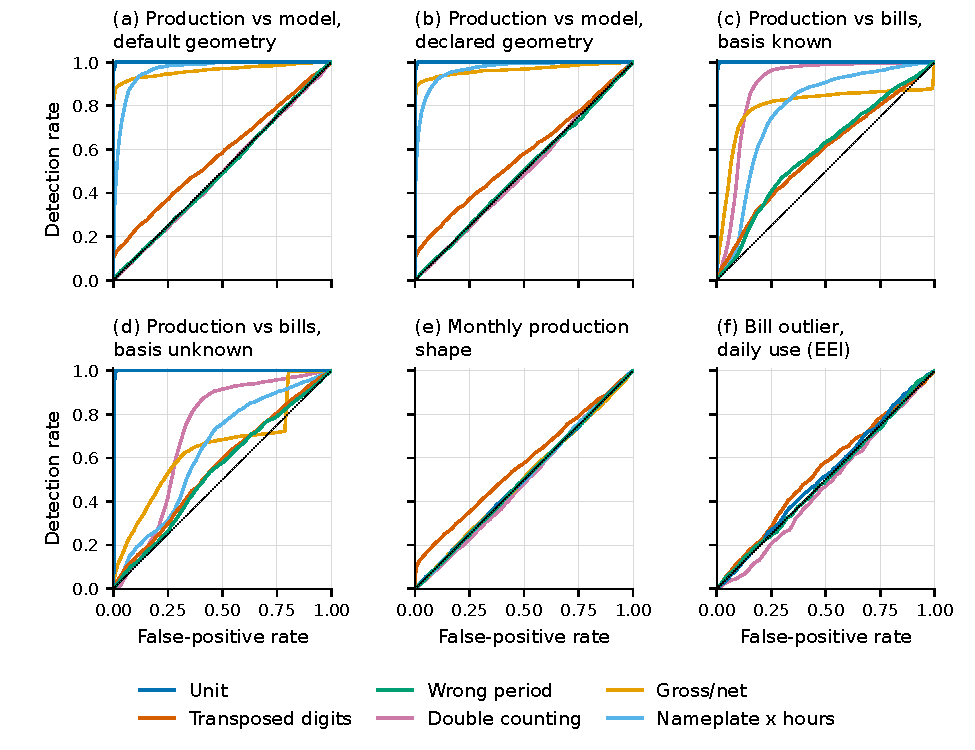
\includegraphics[width=0.9\linewidth]{figures/fig4_validation_roc}
\caption{Synthetic data. ROC curves of the statistical rules by injected error class.}
\end{figure}

\subsection{Accuracy of verification}

\begin{table}[h]
\caption{Synthetic data, error-free evidence. Absolute relative error (\%) of EEI
annual-savings estimators against true normal-year savings ($n=\NEei$).}\label{tab:a3}
\centering\footnotesize
\begin{tabular}{p{0.5\linewidth}rrrr}
\hline
Estimator of annual savings & 5th pct. & Median & 95th pct. & Share $>10\%$ \\
\hline
Undated monthly difference & 2.0 & 22.8 & 100 & 75 \\
Dated, day-annualized difference & 2.0 & 22.5 & 97 & 75 \\
Dated monthly, degree-day normalized & 1.2 & 15.2 & 78 & 64 \\
Dated monthly, normalized when the models meet the fit criterion & 1.1 & 15.2 & 77 & 64 \\
As above, estimated reads merged & 1.1 & 14.5 & 69 & 62 \\
Daily interval data, normalized & 0.9 & 12.1 & 60 & 56 \\
\hline
\end{tabular}

\end{table}

\setcounter{figure}{2}
\begin{figure}[h]
\centering
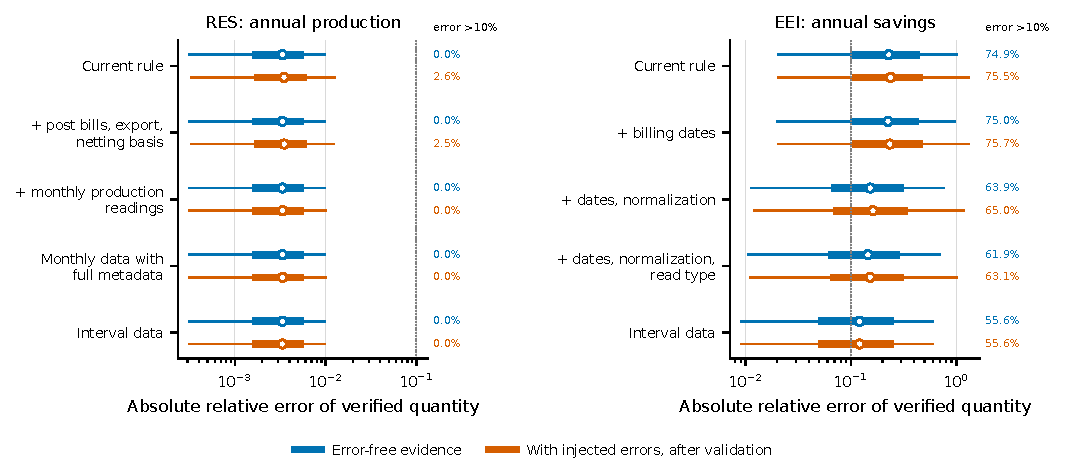
\includegraphics[width=0.95\linewidth]{figures/fig3_error_distributions}
\caption{Synthetic data. Absolute relative error of the verified quantity by evidence
specification (median, interquartile range, 5th--95th percentile; share above 10\% at
right). Blue: error-free evidence. Vermilion: injected errors, after validation.}
\end{figure}

For RES, correctly reported metered production is accurate to about
\AccCurrentCleanResMedian\%; with injected errors the share of applicants more than 10\%
off is \AccCurrentUnvalidatedResShareTen\% without validation,
\AccCurrentValidatedResShareTen\% with the checks possible under the current elements and
\AccProductionMeterValidatedResShareTen\% with monthly production readings. For EEI,
median error falls from \PathUndatedNormalMedian\% (undated difference) to
\PathNormMergedNormalMedian\% (dated bills, read type, guarded adjustment) and
\PathIntervalPathNormalMedian\% (interval data); the root-mean-square error of the
adjusted monthly estimate (\NormEeiNormRmse\% of pre-installation use) is not below that of
the simple difference (\NormEeiRawRmse\%). Nominal \CoverageNominal\% uncertainty intervals
from twelve-point baselines covered the truth in \CoverageFsu\% (Guideline 14 form) and
\CoverageBootstrap\% (block bootstrap) of cases.

\begin{table}[h]
\caption{Synthetic data. Median absolute relative error (\%) of EEI savings estimators by
true savings as a share of pre-installation use.}
\centering\footnotesize
\begin{tabular}{lrrr}
\hline
Estimator & below 10\% & 10-20\% & above 20\% \\
\hline
dated & 32 & 19 & 17 \\
interval & 15 & 9 & 13 \\
normalized guarded & 19 & 13 & 15 \\
normalized merged & 17 & 12 & 15 \\
normalized monthly & 19 & 13 & 15 \\
undated & 33 & 19 & 17 \\
\hline
\end{tabular}

\end{table}

\subsection{Accuracy and burden}

\setcounter{figure}{5}
\begin{figure}[h]
\centering
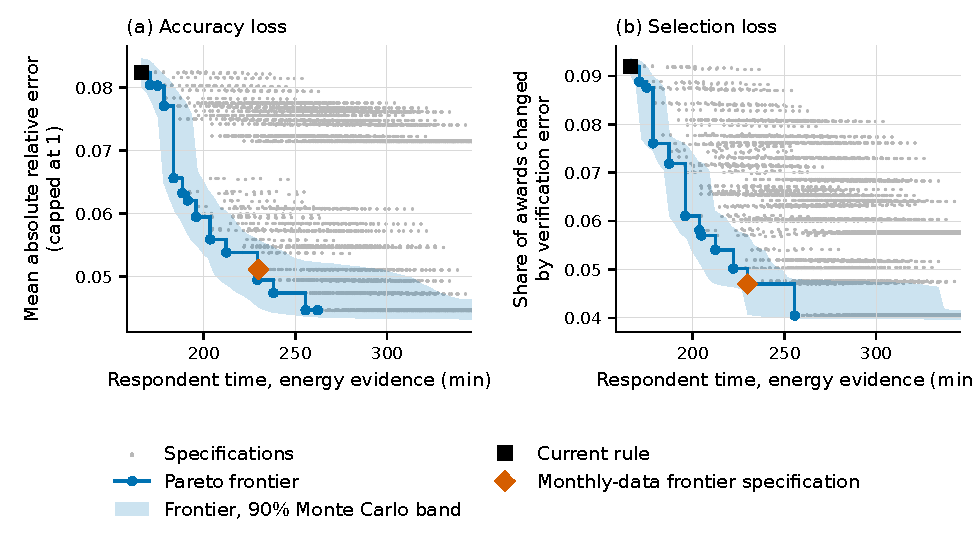
\includegraphics[width=0.95\linewidth]{figures/fig6_frontier}
\caption{Synthetic data, hypothetical element times. All feasible specifications under
manual entry, Pareto frontier with 90\% Monte Carlo band, current rule (square) and
monthly-data frontier specification (diamond).}
\end{figure}

\begin{table}[h]
\caption{Synthetic data, hypothetical element times. Specifications on the accuracy
frontier under manual entry: minutes; accuracy loss overall, RES, EEI (\%); share of
awards changed (\%); errors detected (\%); false-positive rate (\%).}\label{tab:a4}
\centering\scriptsize
\begin{tabular}{p{0.44\linewidth}rrrrrrr}
\hline
Optional elements collected & Min. & MARE & RES & EEI & Sel. & Det. & FP \\
\hline
(current rule) & 166 & 8.2 & 1.0 & 33.4 & 9.2 & 41 & 2.6 \\
enduse share & 171 & 8.0 & 1.0 & 32.5 & 8.9 & 42 & 2.6 \\
pv geometry & 175 & 8.0 & 0.7 & 33.4 & 8.8 & 44 & 3.1 \\
meter ids & 178 & 7.7 & 1.0 & 31.0 & 7.6 & 56 & 2.6 \\
billing dates, weather normalization & 184 & 6.6 & 1.0 & 25.9 & 7.8 & 59 & 2.9 \\
billing dates, enduse share, weather normalization & 188 & 6.3 & 1.0 & 24.8 & 7.4 & 61 & 2.9 \\
billing dates, read type, weather normalization & 191 & 6.2 & 1.0 & 24.3 & 7.5 & 59 & 2.9 \\
billing dates, meter ids, weather normalization & 196 & 5.9 & 1.0 & 23.1 & 6.1 & 75 & 2.9 \\
billing dates, read type, meter ids, weather normalization & 204 & 5.6 & 1.0 & 21.5 & 5.8 & 75 & 2.9 \\
billing dates, read type, meter ids, pv geometry, weather normalization & 212 & 5.4 & 0.7 & 21.5 & 5.4 & 78 & 3.3 \\
utility interval, weather normalization & 229 & 4.9 & 1.0 & 18.6 & 5.2 & 41 & 2.6 \\
pv geometry, utility interval, weather normalization & 238 & 4.7 & 0.7 & 18.6 & 4.8 & 44 & 3.1 \\
inverter monthly, utility interval, weather normalization & 256 & 4.5 & 0.4 & 18.6 & 4.0 & 53 & 3.3 \\
inverter interval, utility interval, weather normalization & 262 & 4.5 & 0.4 & 18.6 & 4.1 & 41 & 2.6 \\
\hline
\end{tabular}

\end{table}

\begin{table}[h]
\caption{Requirement-to-schema traceability by section of 7 CFR part 4280 subpart B.}
\label{tab:a5}
\centering\footnotesize
\begin{tabular}{llrrp{0.34\linewidth}}
\hline
Section & Subject & Paragraphs & Mapped & Schema classes used \\
\hline
\S4280.104 & Definitions & 10 & 10 & BillingRecord, Meter, PerformanceClaim, Project \\
\S4280.122 & Project eligibility & 171 & 46 & BillingRecord, EquipmentItem, Facility, IntervalSeries, Meter, PerformanceClaim, Project \\
\S4280.131 & Application requirements & 73 & 14 & Applicant, BillingRecord, EquipmentItem, Facility, Meter, PerformanceClaim, Project \\
\S4280.160 & Reporting requirements & 3 & 2 & EquipmentItem, PerformanceClaim \\
\hline
\end{tabular}

\end{table}

\begin{table}[h]
\caption{Synthetic data, hypothetical element times. Respondent minutes and losses by
collection mode when the mode is available to every respondent. ``recommended'' is the
monthly-data frontier specification; ``recommended interval'' the frontier specification
when interval data are allowed.}\label{tab:a6}
\centering\footnotesize
\begin{tabular}{llrrrr}
\hline
Specification & Collection mode & Minutes & 90\% interval & MARE (\%) & Selection change (\%) \\
\hline
current & Manual transcription & 166 & 164--170 & 8.2 & 9.2 \\
current & Utility file upload & 103 & 82--132 & 8.2 & 9.2 \\
current & Green Button download & 103 & 82--132 & 8.2 & 9.2 \\
current & Automated utility data access & 82 & 64--104 & 8.2 & 9.2 \\
recommended & Manual transcription & 230 & 211--255 & 5.1 & 4.7 \\
recommended & Utility file upload & 133 & 107--171 & 5.1 & 4.7 \\
recommended & Green Button download & 133 & 107--171 & 5.1 & 4.7 \\
recommended & Automated utility data access & 112 & 89--143 & 5.1 & 4.7 \\
recommended interval & Manual transcription & 256 & 228--340 & 4.5 & 4.0 \\
recommended interval & Utility file upload & 192 & 156--291 & 4.5 & 4.0 \\
recommended interval & Green Button download & 129 & 104--166 & 4.5 & 4.0 \\
recommended interval & Automated utility data access & 108 & 85--138 & 4.5 & 4.0 \\
metadata & Manual transcription & 278 & 251--319 & 5.1 & 4.7 \\
metadata & Utility file upload & 146 & 120--191 & 5.1 & 4.7 \\
metadata & Green Button download & 146 & 120--192 & 5.1 & 4.7 \\
metadata & Automated utility data access & 125 & 102--163 & 5.1 & 4.7 \\
interval & Manual transcription & 262 & 234--351 & 4.5 & 4.1 \\
interval & Utility file upload & 199 & 163--300 & 4.5 & 4.1 \\
interval & Green Button download & 136 & 110--180 & 4.5 & 4.1 \\
interval & Automated utility data access & 115 & 91--150 & 4.5 & 4.1 \\
\hline
\end{tabular}

\end{table}

\subsection{Selection}

\begin{figure}[h]
\centering
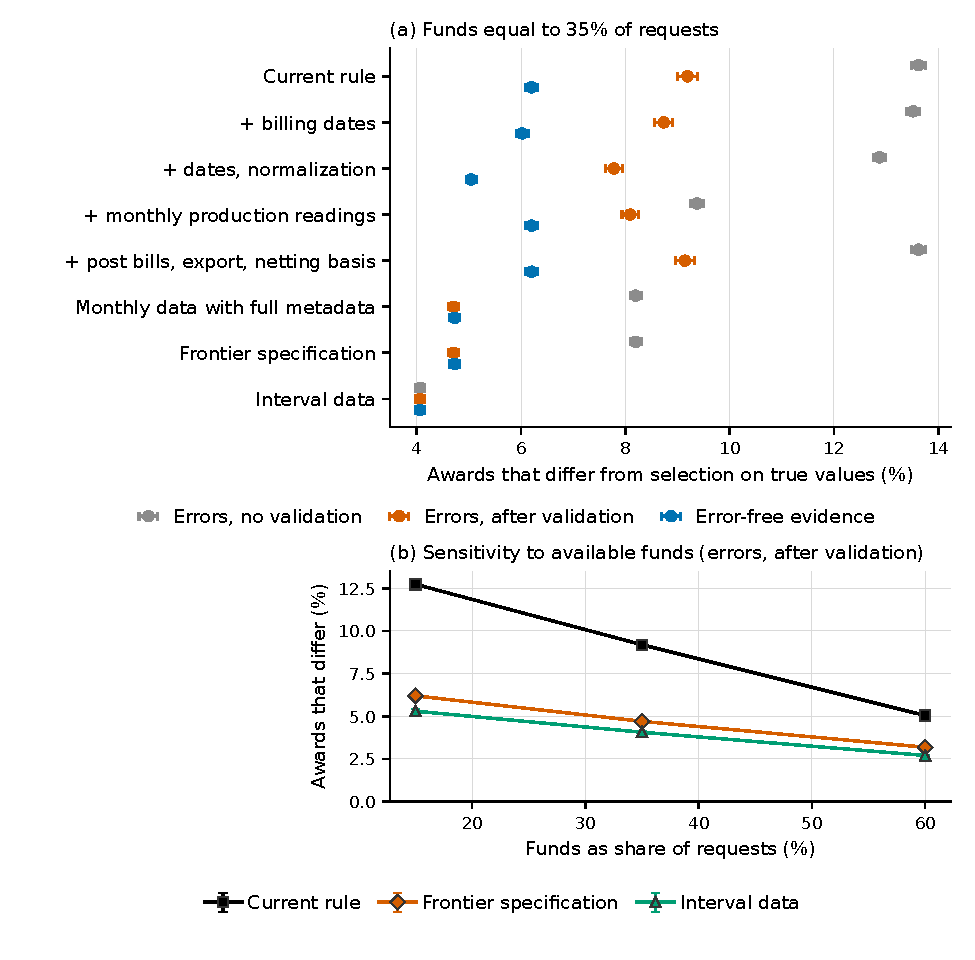
\includegraphics[width=0.9\linewidth]{figures/fig7_selection}
\caption{Synthetic competitions with hypothetical funding and non-energy scores. Share of
awards that differ from selection on true values.}
\end{figure}

In the synthetic population \ShareEnergyCap\% of applications reach the cap of the
energy-per-dollar criterion, so differences in energy-dependent points arise from the
banded percentage and payback criteria. With funds at \FundRatioMid\% of requests the
share of awards changed is \SelCurrentCleanMid\% with error-free evidence,
\SelCurrentValidatedMid\% with errors after validation and \SelCurrentUnvalidatedMid\% with
errors unvalidated under the current elements; \SelRecValidatedMid\% under the
monthly-data frontier specification; \SelIntervalValidatedMid\% with interval data.

\clearpage
\section{Validation status and limitations}

\begin{itemize}
\item \emph{Numerical correctness}: unit and property tests (energy conservation in
billing, recovery of known regression coefficients, agreement with an independent
least-squares implementation, selection invariants, optimizer against enumeration).
\item \emph{Model verification}: the photovoltaic model matches an independent PVWatts v8
run on identical weather within \PvRefAnnualDiff\% annually.
\item \emph{Empirical validity}: not established. No REAP microdata were used and none
are public for the revised rule.
\item \emph{Assumptions}: aggregate commercial load shapes; hypothetical agricultural
shapes, electricity only; photovoltaic RES only; hypothetical noise, error rates, element
times, funding and non-energy points; flagged errors assumed corrected; fabricated
readings not modelled; territories not represented. Monte Carlo standard errors of the
headline losses are below 2\% of their values.
\end{itemize}

\section{Schema element list}

The schema source, JSON Schema, pydantic models and CSV templates are in the repository
directory \texttt{src/reapschema/schema/}. Elements marked ``no'' under Required are
optional in the schema.

{\footnotesize
\begin{longtable}{llllp{0.1\linewidth}}
\caption{Elements of the evidence schema (generated from the LinkML source).}\label{tab:schema}\\
\hline
Class & Element & Range & Required & Unit \\
\hline
\endfirsthead
\hline
Class & Element & Range & Required & Unit \\
\hline
\endhead
Applicant & id & string & yes &  \\
Applicant & legal\_name & string & yes &  \\
Applicant & applicant\_type & ApplicantType & yes &  \\
Applicant & unique\_entity\_identifier & string & no &  \\
Facility & id & string & yes &  \\
Facility & address & string & yes &  \\
Facility & state & string & yes &  \\
Facility & latitude & float & no & deg \\
Facility & longitude & float & no & deg \\
Facility & climate\_zone & integer & no &  \\
Facility & weather\_station\_id & string & no &  \\
Project & id & string & yes &  \\
Project & category & ProjectCategory & yes &  \\
Project & res\_subcategory & ResSubcategory & no &  \\
Project & technology & TechnologyClass & yes &  \\
Project & rated\_capacity & float & no &  \\
Project & rated\_capacity\_unit & PowerUnit & no &  \\
Project & in\_service\_date & date & yes &  \\
Project & project\_period\_start & date & no &  \\
Project & project\_period\_end & date & no &  \\
Project & project\_cost & float & no & [USD] \\
Project & amount\_requested & float & no &  \\
Project & useful\_life\_years & float & no & a \\
Project & array\_tilt & float & no & deg \\
Project & array\_azimuth & float & no & deg \\
Project & storage\_capacity & float & no &  \\
Project & affected\_end\_use\_share & float & no &  \\
Meter & id & string & yes &  \\
Meter & meter\_type & MeterType & yes &  \\
Meter & netting\_arrangement & NettingArrangement & no &  \\
Meter & billed\_quantity\_basis & BilledQuantityBasis & no &  \\
Meter & dedicated & boolean & no &  \\
Meter & utility\_account & string & no &  \\
Meter & interval\_minutes & integer & no &  \\
BillingRecord & meter & Meter & yes &  \\
BillingRecord & is\_pre\_installation & boolean & yes &  \\
BillingRecord & period\_start & date & no &  \\
BillingRecord & period\_end & date & no &  \\
BillingRecord & read\_type & ReadType & no &  \\
BillingRecord & energy\_imported & float & yes &  \\
BillingRecord & energy\_exported & float & no &  \\
BillingRecord & energy\_unit & EnergyUnit & yes &  \\
BillingRecord & peak\_demand & float & no & kW \\
BillingRecord & energy\_charge & float & no & [USD] \\
IntervalSeries & meter & Meter & yes &  \\
IntervalSeries & is\_pre\_installation & boolean & yes &  \\
IntervalSeries & start\_time & datetime & yes &  \\
IntervalSeries & time\_zone & string & yes &  \\
IntervalSeries & interval\_minutes & integer & yes &  \\
IntervalSeries & energy\_unit & EnergyUnit & yes &  \\
IntervalSeries & values & float & yes &  \\
PerformanceClaim & quantity & ClaimQuantity & yes &  \\
PerformanceClaim & claimed\_value & float & yes &  \\
PerformanceClaim & energy\_unit & EnergyUnit & yes &  \\
PerformanceClaim & method & ClaimMethod & no &  \\
PerformanceClaim & normalization\_basis & NormalizationBasis & no &  \\
PerformanceClaim & relative\_uncertainty & float & no &  \\
PerformanceClaim & pre\_period\_energy & float & no &  \\
PerformanceClaim & post\_period\_energy & float & no &  \\
PerformanceClaim & energy\_price & float & no &  \\
EquipmentItem & make & string & yes &  \\
EquipmentItem & model & string & yes &  \\
EquipmentItem & item\_quantity & integer & yes &  \\
EquipmentItem & component\_role & string & no &  \\
EquipmentItem & country\_of\_origin & string & no &  \\
EquipmentItem & acquisition\_cost & float & no &  \\
EquipmentItem & acquisition\_date & date & no &  \\
EvidencePackage & id & string & yes &  \\
EvidencePackage & collection\_mode & CollectionMode & no &  \\
EvidencePackage & applicant & Applicant & yes &  \\
EvidencePackage & facility & Facility & yes &  \\
EvidencePackage & project & Project & yes &  \\
EvidencePackage & meters & Meter & yes &  \\
EvidencePackage & billing\_records & BillingRecord & no &  \\
EvidencePackage & interval\_series & IntervalSeries & no &  \\
EvidencePackage & performance\_claim & PerformanceClaim & yes &  \\
EvidencePackage & equipment & EquipmentItem & no &  \\
\hline
\end{longtable}

}

\bibliographystyle{unsrtnat}
\bibliography{../paper/references}
\end{document}
